
\chapter{Logistic regression}
\label{sec:logit}
Generalized linear models, of which the logit is one, form a large branch of statistical models that seek to use many of the tools of linear regression on dependent variables that do not meet the requirements of OLS regression; namely linearity and normality.

We begin by trying to derive the estimator for a dichotomous outcome, finding we have a problem, then offering a solution. We then move from this specific circumstance to a more general framework of generalized linear models that can encompass many types of outcomes that can be expressed in a specific form.

Consider the data in Table~\ref{tab:logitexample}. Figure~\ref{fig:exlogit1} presents a scatter plot of these data.  How would we best model $y$? One possibility would be to use OLS regression and fit a linear probability model
\[
y_i=\beta_0+\beta_1x_i+e_i
\]
The big problem with this approach is that some values of $x$ produce nonsense values of $y$, as we can see in Figure~\ref{fig:exlogit2}. In this figure, two of the values of $x$ predict values of $y$ that are less than 1, which is out of the range for this type of outcome.

\begin{figure}
   \centering
   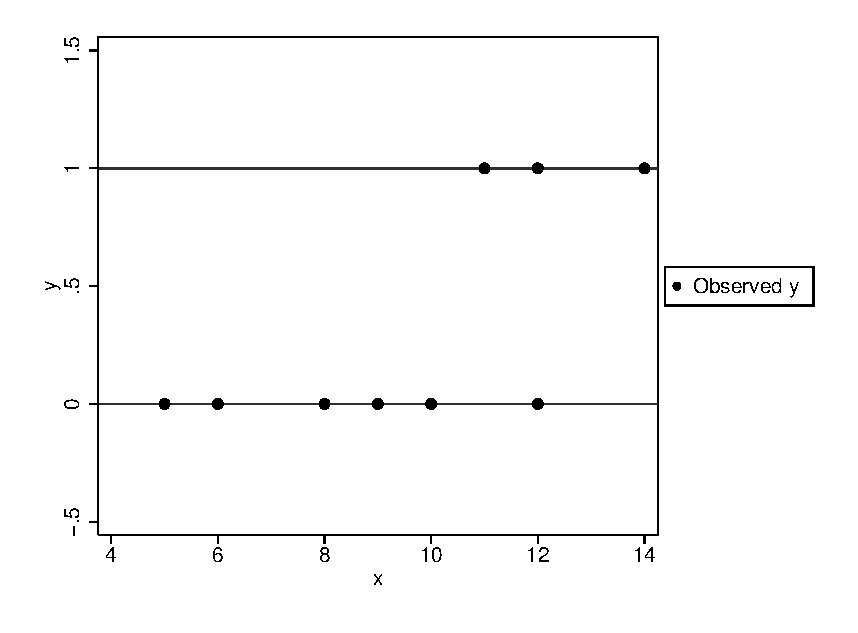
\includegraphics[angle=0,
           width=.75\textwidth]{exlogit1.eps}
   \caption{Scatterplot of data in Table~\ref{tab:logitexample}}
  \label{fig:exlogit1}
\end{figure}

The other more technical problems with this approach is that we don't meet all the assumptions of OLS regression:
\begin{itemize}
\item{$y$ is a linear function of predictors--NO!}
\item{The expected value of any residual is zero--NO!}
\item{The variance of the residuals in constant--NO!}
\item{The covariance of all residuals is zero, i.e. $\mbox{cov}\left(e_i,e_j\right)=0$}
\item{The values of the predictors are not random (especially the intercept)}
\item{The values of the predictors are not linear combinations of each other}
\item{The errors are distributed normally--NO!}
\end{itemize}

\begin{table}[htbp]\centering
\caption{Dichotomous variable $y$ and predictor $x$ \label{tab:logitexample}
\textbf{} }\begin{tabular} {@{} c c @{}} \\
$y$ & $x$ \\
\hline
0&5\\
0&8\\
0&12\\
1&12\\
0&10\\
0&10\\
0&9\\
1&14\\
0&6\\
1&11\\
\hline
\multicolumn{2}{@{}l}{\footnotesize{\emph{} }}
\end{tabular}
\end{table}

\begin{figure}
   \centering
   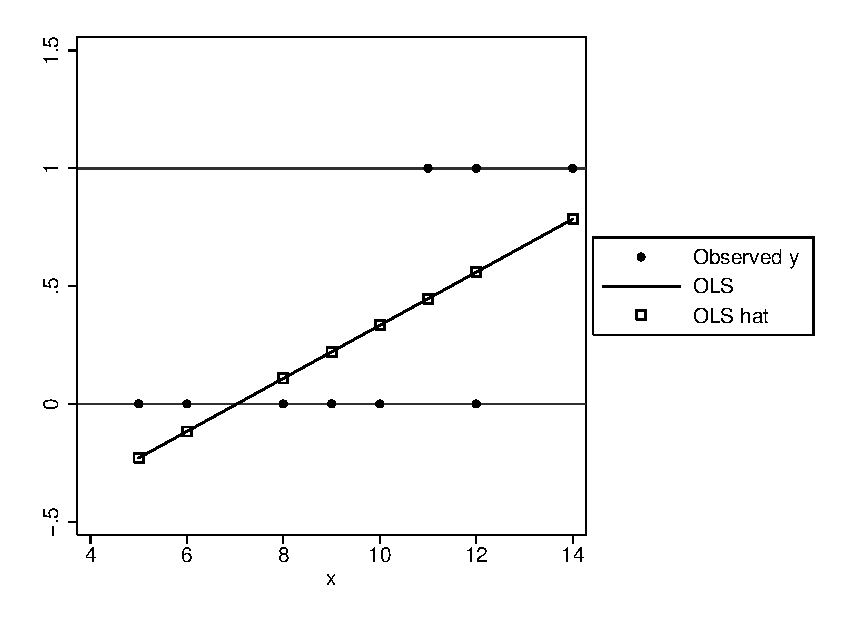
\includegraphics[angle=0,
           width=.75\textwidth]{exlogit2.eps}
   \caption{Scatterplot of data in Table~\ref{tab:logitexample} with linear probability model (OLS)}
  \label{fig:exlogit2}
\end{figure}

\subsection{Dealing with probabilities and odds}

To fit a model with these data, we need to deal with the mean of $y$. Remember that regression is about means, and regression is about predicting the mean of $y$ as a function of covariates. Recall that the mean of a dichotomous variable is a proportion. The issue with regression is that we are constrained by the fact that proportions are bound by 1 and 0, and regressions are infinite lines. The trick is to transform expected (i.e., the mean) outcome into a logit (log odds).

Thus, the mean of $y$ is
\begin{equation}
\bar{y} = \mbox{proportion of 1s} = \mbox{chance of 1s}
\end{equation}
and then the odds are
\[
\mbox{odds} = \frac{\mbox{Chance of something happening}}{\mbox{Chance of something not happening}}
\]
or
\begin{equation}
\mbox{odds} = \frac{\bar{y}}{1-\bar{y}}
\end{equation}
which can be turned into an infinite line with a natural log
\begin{equation}
\mbox{log odds} = \mbox{ln}\left(\frac{\bar{y}}{1-\bar{y}}\right)
\end{equation}

So, let's call the function for the mean of $y$ as a function of $x$ $\pi$. This makes the bivariate regression
\begin{equation}
\mbox{ln}\left(\frac{\pi\left(x\right)}{1-\pi\left(x\right)}\right)=\beta_0+\beta_1x
\end{equation}
This gives us a regression model to fit the log-odds as a function of covariates
\begin{equation}
\mbox{ln}\left(\frac{\mbox{Pr}\left(y_i = 1\right)}{\mbox{Pr}\left(y_i = 0\right)}\right)=\beta_0+\beta_1x
\end{equation}
which we can rearrange to get a function for the mean (i.e. probability) of $y$
\begin{equation}
\pi\left(x\right)=\frac{e^{\beta_0+\beta_1x}}{1+e^{\beta_0+\beta_1x}}
\end{equation}

To summarize, given a mean of $y$, which we will call the probability $p$, we can consider the logit function that produces log-odds (the left panel of Figure~\ref{fig:logitfunction})
\begin{equation}
logit(p) = \mbox{ln}\left(\frac{p}{1-p}\right)
\end{equation}
as the quantity to model, and then once we have the estimates of $\beta_0$ and $beta_1$ that predict the log-odds, we can return to probabilities with the inverse logit function (the right panel of Figure~\ref{fig:logitfunction})
\begin{equation}
inv.logit(\beta_0,\beta_1,x)=\frac{e^{\beta_0+\beta_1x}}{1+e^{\beta_0+\beta_1x}}
\end{equation}

\begin{figure}
   \centering
   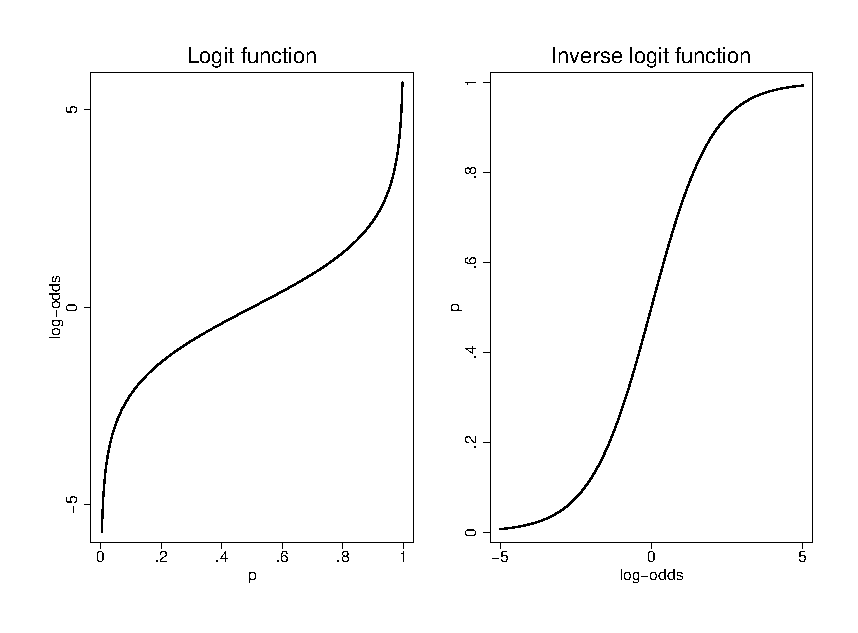
\includegraphics[angle=0,
           width=.75\textwidth]{logitfunction.eps}
   \caption{Logit and inverse-logit functions}
  \label{fig:logitfunction}
\end{figure}

\subsection{Estimating a regression that predicts probabilities and odds}
Recall that the likelihood for a binomial variable is
\[
L\left(p \vert y_1 \ldots y_N\right)=p^{\sum_{i=1}^Ny_i}\left(1-p\right)^{N-\sum_{i=1}^Ny_i}
\]
where $\mbox{Pr}\left(y_i = 1\right) = p$, see ~\eqref{eq:plikelihood}. We can rewrite this as
\begin{equation}
L\left(p_i \vert y_1 \ldots y_N\right)=\prod_{i=1}^N\pi\left(x_i\right)^{y_i}\left(1-\pi\left(x_i\right)\right)^{1-y_i}
\end{equation}
or
\begin{equation}
L\left(p_i \vert y_1 \ldots y_N\right)=\prod_{i=1}^N \left(\frac{\pi\left(x_i\right)}{1-\pi\left(x_i\right)}\right)^{y_i}\left(1-\pi\left(x_i\right)\right)
\end{equation}
Since
\[
\left(\frac{\pi\left(x_i\right)}{1-\pi\left(x_i\right)}\right)=e^{\beta_0+\beta_1x_i}
\]
and
\[
\left(1-\pi\left(x_i\right)\right) = \left(1+e^{\beta_0+\beta_1x_i}\right)^{-1}
\]
then the likelihood is
\begin{equation}
L\left(p_i \vert y_1 \ldots y_N\right)=\prod_{i=1}^N e^{y_i\beta_0+\beta_1x_i}\left(1+e^{\beta_0+\beta_1x_i}\right)^{-1}
\end{equation}
and the log likelihood is
\begin{equation}
\mbox{ln}\left(L\left(p_i \vert y_1 \ldots y_N\right)\right)=\sum_{i=1}^N y_i\left(\beta_0+\beta_1x_i\right)-\mbox{ln}\left(1+e^{\beta_0+\beta_1x_i}\right)
\end{equation}

Now that we have a likelihood function, we {\it should} be able to derive the estimators for the intercept and slope. Let's start with the intercept:
\begin{equation}
\frac{\partial\mbox{ln}\left(L\left(p_i \vert y_1 \ldots y_N\right)\right)}{\partial\beta_0}=\sum_{i=1}^Ny_i-\frac{e^{\beta_0+\beta_1x_i}}{1+e^{\beta_0+\beta_1x_i}}
\end{equation}
set to zero and
\begin{equation}
\sum_{i=1}^Ny_i=\sum_{i=1}^N\frac{e^{\beta_0+\beta_1x_i}}{1+e^{\beta_0+\beta_1x_i}}
\end{equation}
the solution is the sum of $y$'s needs to be the sum of predicted probabilities. Now, for the slope
\begin{equation}
\frac{\partial\mbox{ln}\left(L\left(p_i \vert y_1 \ldots y_N\right)\right)}{\partial\beta_1}=\sum_{i=1}^Nx_iy_i-\frac{x_i}{1+e^{-\beta_0+\beta_1x_i}}
\end{equation}
set to zero and
\begin{equation}
\sum_{i=1}^Nx_iy_i=\sum_{i=1}^N\frac{x_i}{1+e^{-\beta_0+\beta_1x_i}}
\end{equation}
No solution exists.

\section{Introduction to maximum likelihood estimation}

How can we find these parameters? We can take advantage of another problem with non-linear outcomes: the variance is dependent on the mean. For example, the variance of a binomial variable is $\mbox{var}\left(y\right)=\bar{y}\left(1-\bar{y}\right)$ or $\mbox{var}\left(p\right)=p\left(1-p\right)$. We then use the tricks we used to solve non-constant variance (see Chapter~\ref{sec:het}, weighted least squares) iteratively. In matrix notation, one procedure of {\it iterative weighted least squares} is as follows (computers do something slightly different, see Chapter~\ref{sec:chapterglm}
\begin{enumerate}
\item{start with $\beta_0$ = the mean, and $\beta_1$ = 0}
\item{calculate weights based on the variance of the mean. In the case of a binomial outcome, the weight for each case is = $\hat{y}_i\left(1-\hat{y}_i\right)$}, where $\hat{y}_i=\frac{e^{\beta_0+\beta_1x_i}}{1+e^{\beta_0+\beta_1x_i}}$
\item{redo the least squares estimates of $\beta_0$ and $\beta_1$ with the new weights and using the residual $(y_i-\hat{y}_i)$ as the outcome. In matrix notation, this is}
\begin{equation}
{\bf{b}_{l+1}} ={\bf{b}_{l}} + {\bf{\left(X'W_lX\right)^{-1}X'\left(y-\hat{y}_l\right)}}
\end{equation}
\item{Each time, calculate the log-likelihood for the new predictions, using the log-likelihood function specific to the type of outcome. In the case of a binomial outcome, this is $\mbox{ln}\left(L\left(p_i \vert y_1 \ldots y_N\right)\right)=\sum_{i=1}^N y_i\left(\beta_0+\beta_1x_i\right)-\mbox{ln}\left(1+e^{\beta_0+\beta_1x_i}\right)$}
\item{Keep going with steps 2-4 until the changes in the log-likelihood are small}
\end{enumerate}

Once we have the parameters, getting the standard errors of the parameters is pretty easy (with matrix algebra). The Asymptotic (i.e. when the samples are big) distribution of the maximum likelihood estimator of the slopes is
\begin{equation}\label{eq:glmmatrixvar}
\mbox{var}\left({\bf b}\right) = {\bf{\left(X'WX\right)^{-1}}}
\end{equation}
and the square-root of the diagonal elements are the standard errors.

\subsection{Example logistic regression estimation}

While this is boring, it does offer some insight. We begin with the data in Table~\ref{tab:logitexample}. The first step is to estimate the mean of our outcome variable, which in this case is 0.3. Using the likelihood function, we see that the log-likelihood for this data is -6.109. We set the intercept to the log-odds (-0.847) and the slope to 0.

\begin{table}[htbp]\centering
\caption{Results from iteration 0 \label{tab:iteration0}
\textbf{} }\begin{tabular} {@{} c c c c @{}} \\ \hline
 iteration 0 \\ \hline
$y$&$p_0$&$\mbox{ln}(odds_0)$&$ll_0$\\ \hline
0&0.300&-0.847&-0.357\\
0&0.300&-0.847&-0.357\\
0&0.300&-0.847&-0.357\\
1&0.300&-0.847&-1.204\\
0&0.300&-0.847&-0.357\\
0&0.300&-0.847&-0.357\\
0&0.300&-0.847&-0.357\\
1&0.300&-0.847&-1.204\\
0&0.300&-0.847&-0.357\\
1&0.300&-0.847&-1.204\\ \hline
&&log likelihood =& -6.10864 \\ \hline
\multicolumn{4}{@{}l}{\footnotesize{\emph{$\beta_0$ = -.84729786, $\beta_1$ = 0 } }}
\end{tabular}
\end{table}

We then use these proportions to get the variances ($p\left(1-p\right)$) for the weight matrix and crank out
\[
{\bf{b}_{l+1}} ={\bf{b}_{l}} + {\bf{\left(X'W_lX\right)^{-1}X'\left(y-\hat{y}_l\right)}}
\]
the results are in Table~\ref{tab:iteration1}. We see that the predicted probabilities are now different, we have a slope, and the log-likelihood is now up -3.726. We keep going like this, each time getting new variances and slopes, until the log-likelihoods stop changing, see Tables~\ref{tab:iteration2} to ~\ref{tab:iteration6}. I plot the iteration's log-likelihoods in Figure~\ref{fig:iteration}.

\begin{table}[htbp]\centering
\caption{Results from iteration 1 \label{tab:iteration1}
\textbf{} }\begin{tabular} {@{} ccccccc @{}} \\ \hline
 iteration 1  \\ \hline
$y$&$p_0$&$y - p_0$&$var(p_0)$&$p_1$&$\mbox{ln}(odds_1)$&$ll_1$ \\ \hline
0&0.300&-0.300&0.210&0.033&-3.370&-0.034\\
0&0.300&-0.300&0.210&0.147&-1.760&-0.159\\
0&0.300&-0.300&0.210&0.596&0.387&-0.905\\
1&0.300&0.700&0.210&0.596&0.387&-0.518\\
0&0.300&-0.300&0.210&0.335&-0.686&-0.408\\
0&0.300&-0.300&0.210&0.335&-0.686&-0.408\\
0&0.300&-0.300&0.210&0.227&-1.223&-0.258\\
1&0.300&0.700&0.210&0.812&1.460&-0.209\\
0&0.300&-0.300&0.210&0.056&-2.833&-0.057\\
1&0.300&0.700&0.210&0.463&-0.150&-0.771\\
\hline &&&& log likelihood & = & -3.72638 \\
\hline
\multicolumn{7}{@{}l}{\footnotesize{\emph{$\beta_0$ = -6.0527866, $\beta_1$ = .53664833} }}
\end{tabular}
\end{table}


\begin{table}[htbp]\centering
\caption{Results from iteration 2 \label{tab:iteration2}
\textbf{} }\begin{tabular} {@{} ccccccc @{}} \\ \hline
 iteration 2 \\ \hline
$y$&$p_1$&$y - p_1$&$var(p_1)$&$p_2$&$\mbox{ln}(odds_2)$&$ll_2$ \\ \hline
0&0.033&-0.033&0.032&0.004&-5.645&-0.004\\
0&0.147&-0.147&0.125&0.047&-3.003&-0.048\\
0&0.596&-0.596&0.241&0.627&0.520&-0.987\\
1&0.596&0.404&0.241&0.627&0.520&-0.467\\
0&0.335&-0.335&0.223&0.224&-1.241&-0.254\\
0&0.335&-0.335&0.223&0.224&-1.241&-0.254\\
0&0.227&-0.227&0.176&0.107&-2.122&-0.113\\
1&0.812&0.188&0.153&0.907&2.281&-0.097\\
0&0.056&-0.056&0.052&0.008&-4.764&-0.008\\
1&0.463&0.537&0.249&0.411&-0.361&-0.890\\
\hline &&&& log likelihood & = & -3.12144 \\
\hline
\multicolumn{7}{@{}l}{\footnotesize{\emph{$\beta_0$ = -10.047784, $\beta_1$ = .88065271} }}
\end{tabular}
\end{table}


\begin{table}[htbp]\centering
\caption{Results from iteration 3 \label{tab:iteration3}
\textbf{} }\begin{tabular} {@{} ccccccc @{}} \\ \hline
 iteration 3 \\ \hline
$y$&$p_2$&$y - p_2$&$var(p_2)$&$p_3$&$\mbox{ln}(odds_3)$&$ll_3$ \\ \hline
0&0.004&-0.004&0.004&0.000&-7.763&-0.000\\
0&0.047&-0.047&0.045&0.016&-4.132&-0.016\\
0&0.627&-0.627&0.234&0.670&0.710&-1.110\\
1&0.627&0.373&0.234&0.670&0.710&-0.400\\
0&0.224&-0.224&0.174&0.153&-1.711&-0.166\\
0&0.224&-0.224&0.174&0.153&-1.711&-0.166\\
0&0.107&-0.107&0.096&0.051&-2.922&-0.052\\
1&0.907&0.093&0.084&0.958&3.130&-0.043\\
0&0.008&-0.008&0.008&0.001&-6.553&-0.001\\
1&0.411&0.589&0.242&0.377&-0.501&-0.975\\
\hline &&&& log likelihood & = & -2.92932 \\
\hline
\multicolumn{7}{@{}l}{\footnotesize{\emph{$\beta_0$ = -13.815145, $\beta_1$ = 1.2103927} }}
\end{tabular}
\end{table}


\begin{table}[htbp]\centering
\caption{Results from iteration 4 \label{tab:iteration4}
\textbf{} }\begin{tabular} {@{} ccccccc @{}} \\ \hline
 iteration 4 \\ \hline
$y$&$p_3$&$y - p_3$&$var(p_3)$&$p_4$&$\mbox{ln}(odds_4)$&$ll_4$ \\ \hline
0&0.000&-0.000&0.000&0.000&-8.922&-0.000\\
0&0.016&-0.016&0.016&0.009&-4.749&-0.009\\
0&0.670&-0.670&0.221&0.693&0.816&-1.182\\
1&0.670&0.330&0.221&0.693&0.816&-0.366\\
0&0.153&-0.153&0.130&0.123&-1.967&-0.131\\
0&0.153&-0.153&0.130&0.123&-1.967&-0.131\\
0&0.051&-0.051&0.048&0.034&-3.358&-0.034\\
1&0.958&0.042&0.040&0.973&3.598&-0.027\\
0&0.001&-0.001&0.001&0.001&-7.531&-0.001\\
1&0.377&0.623&0.235&0.360&-0.576&-1.022\\
\hline &&&& log likelihood & = & -2.90239 \\
\hline
\multicolumn{7}{@{}l}{\footnotesize{\emph{$\beta_0$ = -15.877707, $\beta_1$ = 1.3911007 } }}
\end{tabular}
\end{table}


\begin{table}[htbp]\centering
\caption{Results from iteration 5 \label{tab:iteration5}
\textbf{} }\begin{tabular} {@{} ccccccc @{}} \\ \hline
 iteration 5 \\ \hline
$y$&$p_4$&$y - p_4$&$var(p_4)$&$p_5$&$\mbox{ln}(odds_5)$&$ll_5$ \\ \hline
0&0.000&-0.000&0.000&0.000&-9.149&-0.000\\
0&0.009&-0.009&0.009&0.008&-4.870&-0.008\\
0&0.693&-0.693&0.213&0.697&0.835&-1.195\\
1&0.693&0.307&0.213&0.697&0.835&-0.361\\
0&0.123&-0.123&0.108&0.117&-2.018&-0.125\\
0&0.123&-0.123&0.108&0.117&-2.018&-0.125\\
0&0.034&-0.034&0.033&0.031&-3.444&-0.031\\
1&0.973&0.027&0.026&0.976&3.687&-0.025\\
0&0.001&-0.001&0.001&0.000&-7.722&-0.000\\
1&0.360&0.640&0.230&0.356&-0.592&-1.032\\
\hline &&&& log likelihood & = & -2.90169 \\
\hline
\multicolumn{7}{@{}l}{\footnotesize{\emph{$\beta_0$ = -16.279248, $\beta_1$ = 1.4261493} }}
\end{tabular}
\end{table}

\begin{table}[htbp]\centering
\caption{Results from iteration 6 \label{tab:iteration6}
\textbf{} }\begin{tabular} {@{} ccccccc @{}} \\ \hline
 iteration 6 \\ \hline
$y$&$p_5$&$y - p_5$&$var(p_5)$&$p_6$&$\mbox{ln}(odds_6)$&$ll_6$ \\ \hline
0&0.000&-0.000&0.000&0.000&-9.155&-0.000\\
0&0.008&-0.008&0.008&0.008&-4.874&-0.008\\
0&0.697&-0.697&0.211&0.697&0.835&-1.195\\
1&0.697&0.303&0.211&0.697&0.835&-0.360\\
0&0.117&-0.117&0.104&0.117&-2.019&-0.125\\
0&0.117&-0.117&0.104&0.117&-2.019&-0.125\\
0&0.031&-0.031&0.030&0.031&-3.447&-0.031\\
1&0.976&0.024&0.024&0.976&3.689&-0.025\\
0&0.000&-0.000&0.000&0.000&-7.728&-0.000\\
1&0.356&0.644&0.229&0.356&-0.592&-1.032\\
\hline &&&& log likelihood & = & -2.90169 \\
\hline
\multicolumn{7}{@{}l}{\footnotesize{\emph{$\beta_0$ = -16.291254, $\beta_1$ = 1.4271929} }}
\end{tabular}
\end{table}

\begin{figure}
   \centering
   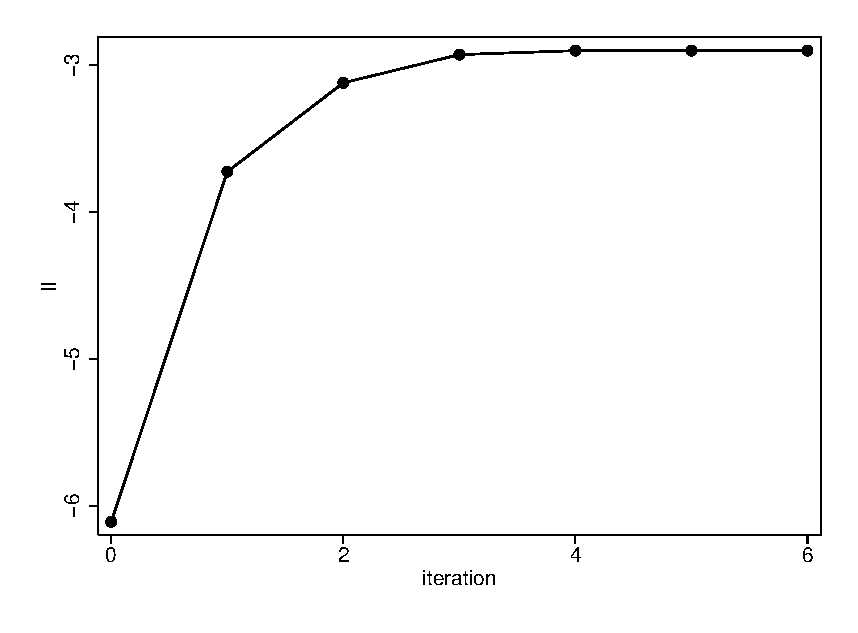
\includegraphics[angle=0,
           width=.75\textwidth]{iteration.eps}
   \caption{Log-likelihoods from maximum likelihood iterations to fit logistic regression to data in Table~\ref{tab:logitexample}}
  \label{fig:iteration}
\end{figure}


With our logistic regression in hand, ($\beta_0$ = -16.291254, $\beta_1$ = 1.4271929), we can now predict the probability of $y=1$ with
\begin{equation}
\hat{p}_i = \frac{e^{\beta_0+\beta_1x_i}}{1+e^{\beta_0+\beta_1x_i}}
\end{equation}
These values are plotted in Figure~\ref{fig:exlogit3}. Notice how the regression line does not cross 0 or 1, unlike Figure~\ref{fig:exlogit2}.

\begin{figure}
   \centering
   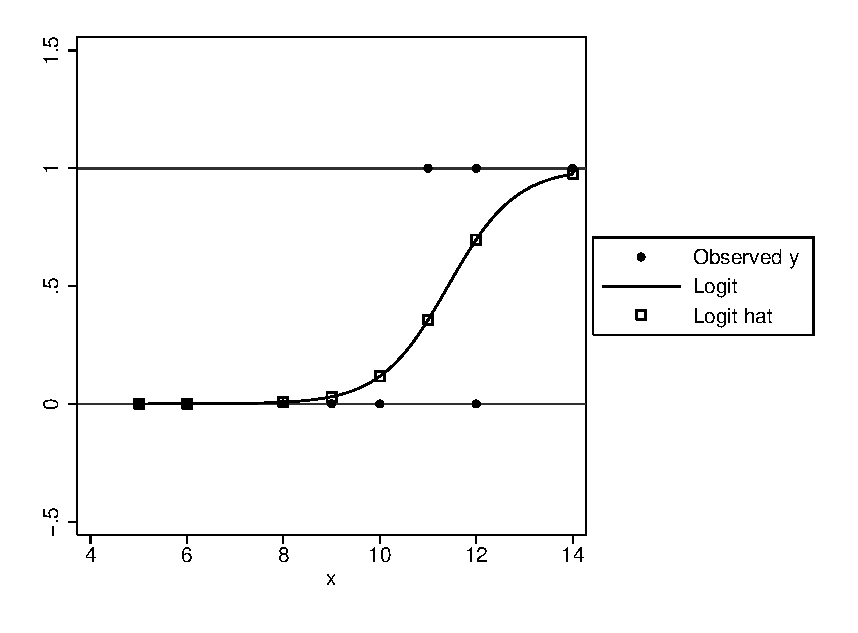
\includegraphics[angle=0,
           width=.75\textwidth]{exlogit3.eps}
   \caption{Scatterplot of data in Table~\ref{tab:logitexample} with logistic regression model}
  \label{fig:exlogit3}
\end{figure}

\subsection{Model statistics}

Models can then be summarized as having good or poor “fit” by looking at the "deviance". The model deviance is
\begin{equation}
G^2 = -2\mbox{ln}\left(L\right)
\end{equation}
We can use this quantity to get a measure of model fit. This is measure is a pseudo-$R^2$. The idea behind this measure is that we measure how much "deviance" we remove by fitting our model. If we use the log-likelihood from iteration 0 ($\mbox{ln}\left(L_0\right)$) and the log-likelihood from the final iteration ($\mbox{ln}\left(L_f\right)$), we can think of the pseudo-$R^2$ as
\begin{equation}
R^2_{pseudo}=1-\frac{G^2_f}{G^2_0}=1-\frac{\mbox{ln}\left(L_f\right)}{\mbox{ln}\left(L_0\right)}
\end{equation}
Another way to think about model fit is with a $\chi^2$ statistic
\begin{equation}
\chi^2 = -2\left(\mbox{ln}\left(L_0\right)-\mbox{ln}\left(L_f\right)\right)
\end{equation}
with degrees of freedom equal to predictors, excluding the constant. Why excluding the constant, because we use the constant in the null (0) model, and this $\chi^2$ statistic reflects how much the likelihood function "improved" with our extra parameters. In other words, its a likelihood ratio test (see Chapter~\ref{sec:lrtest})!

This is another method to test the model. Recall that the likelihood for the null model above (Table ~\ref{tab:iteration0}) was -6.10864, and that by iteration 6, (Table ~\ref{tab:iteration6}) was -2.90169. This leads to a $\chi^2$ of
\[
\chi^2 = -2((-6.10864)-(-2.90169)) = 6.4139
\]
which is significant with 1 degree of freedom.

In the model, the slope is $\beta_1$ = 1.4271929 with a standard error (see next section) of 0.9986. This leads to a test statistic of
\[
z = 1.4271929/0.9986 = 1.4292
\]
Not significant. Unlike OLS regression, the test of the significance for model fit does not directly relate to the test of coefficients.

\subsection{Variances of slopes}

Without getting {\it too} technical, the variance of the slopes is related to the curvature of the likelihood function at the end of the iterations. In other words, it is related to how "flat" the function is at that point. When it is very flat, the estimates are uncertain and the standard errors are large. If it less flat, and more of a tip, the estimate is precise, and the standard errors are small. The mechanics of how this works is a little beyond the scope of these notes, but the foregoing discussion should shed some intuitive light.

If you compare Figure~\ref{fig:iteration} with Figure~\ref{fig:ll}, you will notice that the plot of iterations looks very similar to the left portion of the likelihood function. How "flat" this region is when the iteration stops is what drives the standard errors. To better understand this, recall that the variance of a proportion is ~\eqref{eq:pvar}
\[
\mbox{var}\left(p\right) = \frac{p\left(1-p\right)}{N}
\]
As with all standard errors, this depends on the variance, which in this case is $p\left(1-p\right)$ and the sample size $N$. Note that the variance is a function of the mean, $p$. The shape of the likelihood function is also a function of $p$, as you recall from Chapter~\ref{sec:pml}. This leads to the intuition that the variance is linked to the shape of the likelihood function.

If you examine Figure~\ref{fig:MLse} you will notice a few things. First, for any value of $p$, the shape of the likelihood function is the same. However, as you increase sample size (going down the rows), the variance of $p$ decreases, leading to a more precise estimate. We expect this. But notice what happens when you stay with the same sample size, but change the value of $p$: as $p$ moves to 0.50, the variance {\it increases}!

\begin{figure}
   \centering
   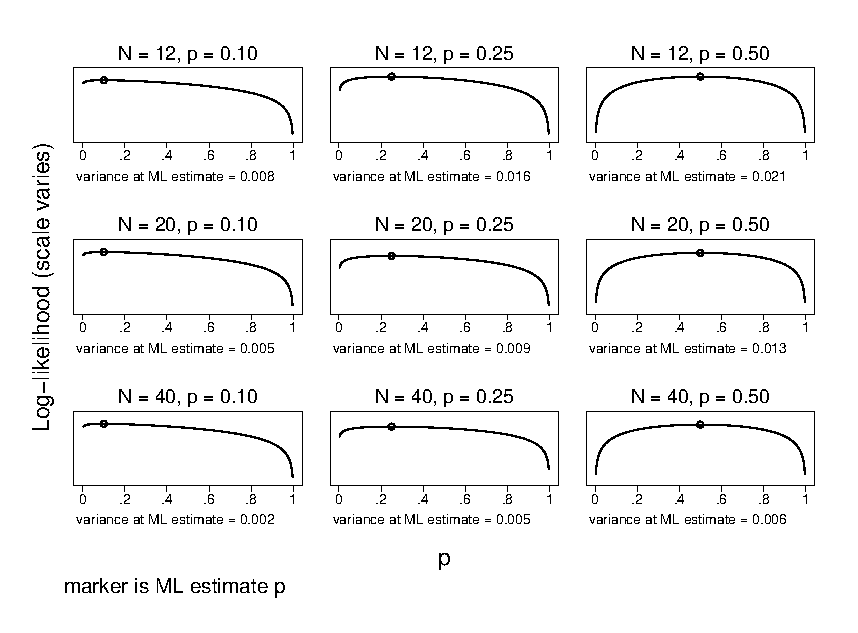
\includegraphics[angle=0,
           width=.75\textwidth]{MLse.eps}
   \caption{Variance of proportion estimator and likelihood functions for various proportions and sample sizes}
  \label{fig:MLse}
\end{figure}

Why does it increase? It depends on how "flat" the likelihood curve is around the estimate. If we zoom in on a row in Figure~\ref{fig:MLse}, instead assuming 100 cases, we get Figure~\ref{fig:MLsezoom}. Notice how the tip of the curve for $p = 0.10$ is "sharp", then how the tip of the curve for $p = 0.50$ is "not as sharp." This "sharpness" is reflected in the variances of the point estimate, which is related directly to what that point estimate actually is; this is different than normal data, where the means and variances are independent.

To connect everything, recall the matrix formula for the variances of the slopes ~\eqref{eq:glmmatrixvar}
\[
\mbox{var}\left({\bf b}\right) = {\bf{\left(X'WX\right)^{-1}}}
\]
what is ${\bf W}$ again? The variances of the predictions for each case ($\hat{p}_i\left(1-\hat{p}_i\right))$! Thus, the standard errors for a logistic regression are based on the variances of the predictions.

Since the concept of degrees of freedom for logistic models is difficult, what many people do is a Wald test for the coefficients. That is, we simply use the $z$ distribution to evaluate the null hypothesis:
\[
z = \frac{\beta}{SE\left(\beta\right)}
\]
where
\[
SE\left(\beta\right) = \sqrt{\mbox{var}\left(\beta\right)}
\]

\begin{figure}
   \centering
   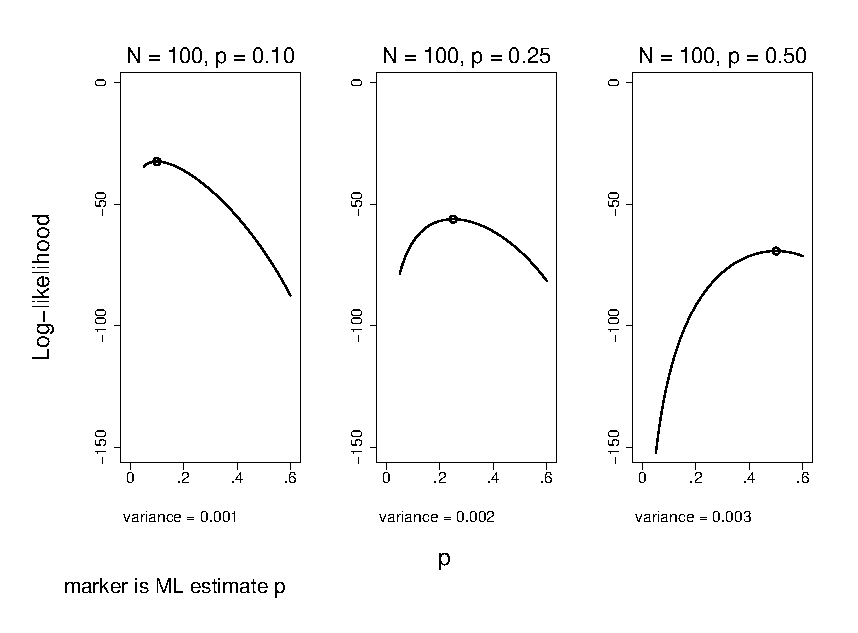
\includegraphics[angle=0,
           width=.75\textwidth]{MLsezoom.eps}
   \caption{Variance of proportion estimator and likelihood functions for various proportions and sample sample size = 100}
  \label{fig:MLsezoom}
\end{figure}

\subsubsection{More technical}

With Figure~\ref{fig:MLsezoom} we can see that the variance is related to the curvature of the likelihood function, or the second derivative. We can see this by taking the second derivative of the likelihood function for the intercept
\[
\frac{\partial^2\mbox{ln}\left(L\right)}{\partial\beta_0^2}=-\sum_{i=1}^N\frac{e^{-\left(\beta_0+\beta_1x_i\right)}}{\left(1+e^{-\left(\beta_0+\beta_1x_i\right)}\right)^2}
\]
which reduces to
\begin{equation}
\frac{\partial^2\mbox{ln}\left(L\right)}{\partial\beta_0^2}=-\sum_{i=1}^N\hat{p}_i\left(1-\hat{p}_i\right)
\end{equation}
and for the slope
\[
\frac{\partial^2\mbox{ln}\left(L\right)}{\partial\beta_1^2} = -\sum_{i-1}^N\left(x_i^2\left(\frac{e^{\beta_0+\beta_1x_i}}{1+e^{\beta_0+\beta_1x_i}}\right)\left(1-\frac{e^{\beta_0+\beta_1x_i}}{1+e^{\beta_0+\beta_1x_i}}\right)\right)
\]
which reduces to
\begin{equation}
\frac{\partial^2\mbox{ln}\left(L\right)}{\partial\beta_1^2}=-\sum_{i=1}^Nx_i^2\hat{p}_i\left(1-\hat{p}_i\right)
\end{equation}
Also, covariance is related to
\begin{equation}
\frac{\partial^2\mbox{ln}\left(L\right)}{\partial\beta_0\beta_1}=-\sum_{i=1}^Nx_i\hat{p}_i\left(1-\hat{p}_i\right)
\end{equation}
As you can see, the curvature of the function is directly related to the variance of the prediction in both cases. These second derivatives of the squared slopes $(\beta_0^2)$ and $(\beta_1^2)$, as well as the product, $(\beta_0\beta_1)$, are formed into what is called a Hessian matrix which is computed with ${\bf{X'WX}}$.
The inverse of ${\bf{X'WX}}$ provides the variances and covariances. This is why the curvature of the likelihood estimation function drives the standard errors of the slopes.

\section{Interpretation}

The core of interpretation in {\it any} regression is the unit of the outcome. In the case of logistic regression the outcome is not a probability, but the log-odds. Thus, the coefficients are in the units of log-odds.

The way to interpret each coefficient is as change in the log-odds. However, log-odds doesn’t have any intrinsic meaning. Instead, it makes more sense to talk about an odds-ratio. This is the ratio the represents what happens when $x$ increases by a single unit. In other words, there are the odds for a value of $x$, and there are the odds for a value $x+1$, what is the ratio between the two? The answer is the exponent of the slope for $x$, $e^{\beta}$.

This is easier to understand with an example. Suppose a simple model where $x$ is coded as either 0 or 1 and the outcome $y$, of course, is coded as 0 or 1. We can think of this as a two by two table as in Table~\ref{tab:2by2}. We can think of the odds that $y$ = 1 given $x$ = 0 as
\begin{equation}
\mbox{odds}\left(y = 1| x = 0\right) = \frac{n_{2,1}/n_{+,1}}{n_{1,1}/n_{+,1}}
\end{equation}
and the odds that $y$ = 1 given that $x$ = 1 as
\begin{equation}
\mbox{odds}\left(y = 1| x = 1\right) = \frac{n_{2,2}/n_{+,2}}{n_{1,2}/n_{+,2}}
\end{equation}
the ratio of these odds works out to
\begin{equation}
\mbox{odds-ratio} = \frac{n_{2,2}/n_{1,2}}{n_{2,1}/n_{1,1}} = \frac{38/7}{14/41} = 15.898
\end{equation}

\begin{table}[htbp]\centering
\caption{Simple 2$\times$2 table \label{tab:2by2}
\textbf{} }\begin{tabular} {@{} cccc @{}} \\
$y$/$x$ & 0 & 1 & total \\ \hline
0 & 41 ($n_{1,1}$) & 7 ($n_{1,2}$) & 48 ($n_{1,+}$) \\
1 & 14 ($n_{2,1}$) & 38 ($n_{2,2}$) & 52 ($n_{2,+}$) \\ \hline
total & 55 ($n_{+,1}$) & 45 ($n_{+,2}$) & 100 ($n_{+,+}$) \\
\end{tabular}
\end{table}

If we had the actual dataset of 100 cases, we could run a logistic regression
\[
\mbox{ln}\left(\frac{\mbox{Pr}\left(y_i = 1\right)}{\mbox{Pr}\left(y_i = 0\right)}\right)=\beta_0 + \beta_1x_i
\]
\[
\mbox{ln}\left(\frac{\mbox{Pr}\left(y_i = 1\right)}{\mbox{Pr}\left(y_i = 0\right)}\right)=-1.074515 + 2.766191x_i
\]
which would produce an estimate of $\beta_1 = 2.766191$, and $e^{2.766191}=15.898$. How is this the case. Again, it comes back to logs. We can write it out like this
\[
\mbox{ln}\left(\mbox{odds}_{x=1}\right) - \mbox{ln}\left(\mbox{odds}_{x=0}\right) = \left(\beta_0+\beta_1\right) - \beta_0 = \beta_1
\]
take the exponent of both sides
\[
\mbox{exp}\left[\mbox{ln}\left(\mbox{odds}_{x=1}\right) - \mbox{ln}\left(\mbox{odds}_{x=0}\right)\right] = \mbox{exp}\left[\beta_1\right]
\]
\begin{equation}\label{eq:oddsratio}
\frac{\mbox{odds}_{x=1}}{\mbox{odds}_{x=0}} = \mbox{exp}\left[\beta_1\right]
\end{equation}
Thus, the exponent of the slope literally is the ratio of the odds. The log odds for $x=0$ is the intercept, -1.074515, which equals odds of 0.34146. The odds for $x=1$ is -1.074515 + 2.766191 = 1.691676, which equals odds of 5.42857. The ratio is 5.42857/0.34146 = 15.898. The nice thing is that this works with continuous (predictor) variables as well.

\subsubsection{Language}

For example, say the odds-ratio is 1.2, then the odds of the outcome being coded "1" is 120 percent as coded "0." Since "120 percent of the odds" is still clumsy, we can take out the "of the odds" by subtracting 1.00 from the odds ratio and replace it with "more odds". Thus, with an odds-ratio of 1.2 we can say: It is 20 percent more odds to get a code of "1" than a code of "0."

If the odds-ratio is 1.00, then the odds of "1" is 100 percent the odds of "0"—the same odds, so equal chances, no effect.

If the odds-ratio is less than 1.0, we can use similar language. Say the odds-ratio is 0.8. Then we can say that the outcome being coded "1" is 80 percent the odds as coded "0." "80 percent the odds" means less odds of "1."  However, “80 percent the odds” is clumsy as well. One thing you can do is subtract the odds ratio from 1.00 and say that the odds of a "1" code is so much less likely. With an odds-ratio is 0.80, 1.00-0.80 = 0.20, so a code of "1" has 20 percent fewer odds.

\subsubsection{Warning!}

I was careful not to use the word {\it chance}. "Chance" often connotes probabilities, and while it is technically not wrong to talk about chance (odds are chances as well), an odds-ratio does not deal with probability. For example, the chance in Table~\ref{tab:2by2} of $y=1|x=0$ is about 25 percent (0.25). The chance of $y=1|x=1$ is about 84 percent (0.84). Taking the ratio, 0.84/0.25 = 3.360. This is a lot different than the {\it odds}-ratio of 15.898. The sloppy report or paper will say the chances increased by 16 fold, putting the idea in people's minds that the probabilities increased 1600 percent--not true!

\subsection{Example logit}

In this section we consider whether some basic covariates impact the opinions of a controversial Arizona law.  SB1070, as the law is commonly known, was passed in Arizona in 2010 and was intended to curb the influx of illegal migrants into the state. One of the provisions was the ability of law enforcement to legally stop and question anyone they suspected of being in the state illegally. Obviously, this stirred a bit of controversy at the time and led to some data collection.  In the analysis below, we consider what demographic and political characteristics of individuals lend themselves to supporting the "stop and question" (SandQ) portion of the law. The descriptive statistics are presented in Table~\ref{tab:sb1070des}.

\begin{table}[htbp]\centering
\caption{Summary statistics of SB1070 poll\label{tab:sb1070des}
\textbf{} }\begin{tabular} {@{} l cccccc @{}} \\ \hline
\textbf{} & {Approve} & {Years} & {Age} & { Female} & {Rep.} & {Dem.} \\
N = 562 & SandQ & {of Educ.} & {$<60$} & \textbf{} & \textbf{ } & \textbf{ } \\
\hline
      Mean(not approve) &   &   15.497 &   0.497 &   0.644 &   0.181 &   0.520 \\
     SD(not approve)   &   &   2.389 &   &   &   &   \\ \\
     Mean(approve)  &   &   14.460 &   0.488 &   0.566 &   0.504 &   0.184 \\
     SD(approve)   &   &   2.167 &   &   &   &   \\ \\
    Mean(all) &   0.685 &   14.786 &   0.491 &   0.591 &   0.402 &   0.290 \\
     SD(all)   &   &   2.289 &   &   &   &   \\
\hline
\multicolumn{7}{@{}l}{
\footnotesize{\emph{Source:} Morrison Institute, Arizona State University}}
\end{tabular}
\end{table}

We see that in this sample, nearly 70 percent of the sample approve of this provision. We also see that the years of education of those that do not approve is a year higher than those who approve. we also see that of those that do not approve, about half are Democrats, and of those that approve, about half are Republican (the reference group is independent).

Next, we fit the model to this data, and the results are presented in Table~\ref{tab:sb1070logit}. Looking at years of education (centered on high school), we see that the log odds decrease by 0.210 for each year of education; the result is significant. Taking the exponent of this, we see that this leads to a decrease in the odds of about 20 percent, again for each year of education. Age and female are not significant.

However, Republicans are far more likely than independents to approve of the provision. The log odds increase by almost 1 when comparing Republicans to independent voters. This leads to an odds ratio of about 2.7. There is an equal and opposite effect for being a Democrat, with the log odds decreasing by 1, leading to a 66 percent reduction in the odds.

The pseudo-$R^2$ is about 0.15, meaning that the likelihood function improved by about 15 percent. The likelihood ratio test is about 104, and with 5 degrees of freedom the model is highly significant.


\begin{table}[htbp]\centering
 \caption{Logistic regression model predicting approval of Arizona SB1070 law provision of questioning
\label{tab:sb1070logit}}
\begin{tabular}{lcc}
\hline
Variable      &    Model & Odds-Ratio  \\
\hline
Year of education - 12    &   -0.210***&    0.811***\\
      &   (0.044)  &   (0.036)  \\
Age LT 60    &   -0.063  &    0.939  \\
      &   (0.204)  &   (0.192)  \\
Female   &   -0.274  &    0.760  \\
      &   (0.210)  &   (0.159)  \\
Republican    &    0.988***&    2.685***\\
      &   (0.258)  &   (0.692)  \\
Democrat    &   -1.069***&    0.343***\\
      &   (0.238)  &   (0.082)  \\
Intercept    &    4.143***&   \\
      &   (0.721)  &   \\
\hline
\multicolumn{1}{l}{Model Statistics} \\
\hline
N      &   562.000  \\
Log-likelihood (null model)    &  -350.127  \\
Log-likelihood (final model)     &  -298.060  \\
Pseudo-$R^2$    &    0.149  \\
$\chi^2 LR$    &   104.133  \\
$df$ Regression    &    5.000  \\
\hline
\multicolumn{1}{l}{$SE$s in parentheses, $***p<0.001$} \\
\hline
\end{tabular}
\end{table}

\subsection{Marginal predictions}

Usually what policy makers want to know is the difference in terms of probability, not odds.  This can be a tricky business because while differences in log odds are linear, and thus constant no matter the reference point, this is not the case with probabilities. Going back to our SB1070 model (Table~\ref{tab:sb1070logit}), we can calculate the predicted probability by simply using the regression model to calculate the log odds, then using the inverse logistic function on the log odds.

For example, the intercept of the model in Table~\ref{tab:sb1070logit} is 4.143, and given the coding of the variables, this represents a male independent voter, with 12 years of education, who is aged 60 or older, which works out to a probability of $e^{4.143}/\left(1+e^{4.143}\right) = 0.9844$. This is represented in Figure~\ref{fig:sb1070hs}, which shows right side of the logit curve with points marked for independents, republicans, and democrats, all assuming older, high school aged, male populations. These numbers are literally just plugging in the coefficients. For example, the log odds for democrats is 4.143-1.069 = 3.074, which translates into a probability of $e^{3.074}/\left(1+e^{3.074}\right) = 0.9558$. Thus, for older males with high school educations, the marginal difference in probabilities is 0.9558 - 0.9844 = 0.0286, or about 3 percentage points.

Next, we alter another parameter and reevaluate these marginal changes. For each year of education the log odds decrease by -0.210, so moving from a high school to a college degree decreases the log odds by $-0.210\times4 = -0.84$ We then shift all the predicted log odds by this amount and recalculate the differences between the political identities. These are presented in Figure~\ref{fig:sb1070col}. Notice that the spacing in the vertical lines is the same as in Figure~\ref{fig:sb1070hs}, but the difference in the horizontal lines (the differences in the probabilities) are different. Now, the effect of being a democrat is about 3 percentage points. In other words, when thinking about probabilities, the effect of political affection is twice as large for the college education as for the high school educated. Assumptions make a difference!


\begin{figure}
   \centering
   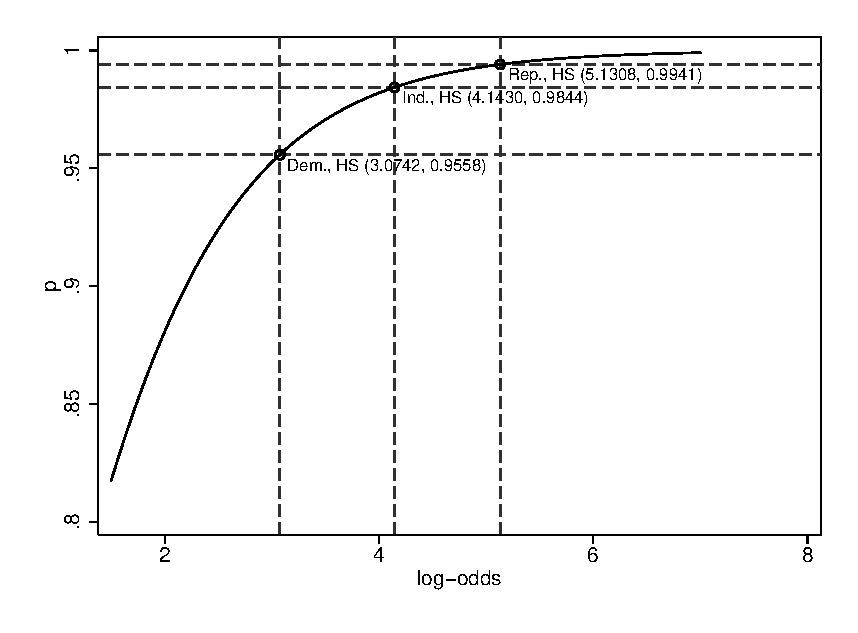
\includegraphics[angle=0,
           width=.75\textwidth]{sb1070hs.eps}
   \caption{Predictions of the probability of approval of Arizona law based on model in Table~\ref{tab:sb1070logit} (12 years of education, male, older population)}
  \label{fig:sb1070hs}
\end{figure}


\begin{figure}
   \centering
   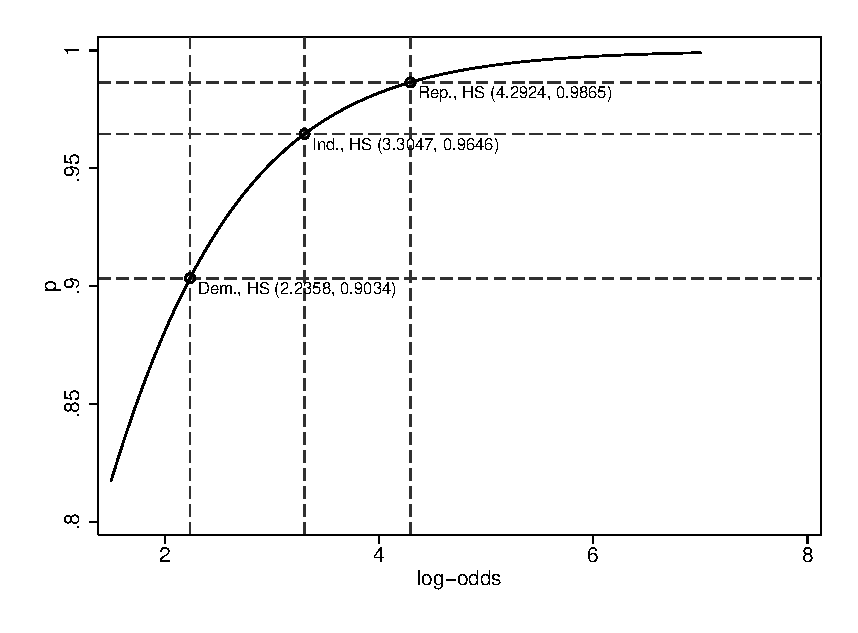
\includegraphics[angle=0,
           width=.75\textwidth]{sb1070col.eps}
   \caption{Predictions of the probability of approval of Arizona law based on model in Table~\ref{tab:sb1070logit} (16 years of education, male, older population)}
  \label{fig:sb1070col}
\end{figure}